\documentclass[12pt]{article}
\usepackage{../lp,graphicx,amsmath}
\usepackage{tkz-berge}
% Cross-references for handout numbers.
\usepackage{amsfonts}
%\usepackage{amsthm}
\usepackage{hyperref}
\usepackage{amssymb}
%\usepackage[capitalize]{cleveref}
\usepackage{xcolor}

%\input{handouts}

\newcounter{chapnum}

\newtheorem{definition}{Definition}[chapnum]
\newtheorem{remark}{Remark}[chapnum]
\newtheorem{theorem}{Theorem}[chapnum]
\newtheorem{lemma}[theorem]{Lemma}
\newtheorem{corollary}[theorem]{Corollary}
\newtheorem{proposition}[theorem]{Proposition}
\newtheorem{claim}[theorem]{Claim}
\newtheorem{observation}{Observation}[chapnum]

\renewcommand{\thesection}{\arabic{chapnum}.\arabic{section}}
\renewcommand{\thefigure}{\arabic{chapnum}.\arabic{figure}}


\newenvironment{proof}{\noindent{\bf Proof:} \hspace*{1em}}{
        \hspace*{\fill} $\triangle$ }
\newenvironment{proof_of}[1]{\noindent {\bf Proof of #1:}
        \hspace*{1em} }{\hspace*{\fill} $\triangle$ }
\newenvironment{proof_claim}{\begin{quotation} \noindent}{
        \hspace*{\fill} $\diamond$ \end{quotation}}
\newenvironment{solution}{\noindent{\bf Solution:} \hspace*{1em}}{
        \hspace*{\fill} $\triangle$ }


\newcommand{\R}{{\mathbb R}}
\newcommand{\Z}{{\mathbb Z}}
\newcommand{\Q}{{\mathbb Q}}
\newcommand{\C}{{\mathbb C}}
\newcommand{\N}{{\mathbb N}}
\newcommand{\lin}{\operatorname{lin}}
\newcommand{\aff}{\operatorname{aff}}
\newcommand{\cone}{\operatorname{cone}}
\newcommand{\conv}{\operatorname{conv}}
\newcommand{\vol}{\operatorname{vol}}
\newcommand{\poly}{\operatorname{poly}}




\newcommand{\CF}[1]{{\color{purple}[CF: #1]}}


\newlength{\toppush}
\setlength{\toppush}{2\headheight}
\addtolength{\toppush}{\headsep}

\newcommand{\htitle}[2]{\noindent\vspace*{-\toppush}\newline\parbox{6.5in}
{Massachusetts Institute of Technology \hfill 18.453: Combinatorial Optimization 
\newline
\textbf{Instructor:} Cole Franks \quad \textbf{Notes: }Michel Goemans and Zeb Brady \hfill#2\newline
\mbox{}\hrulefill\mbox{}}\vspace*{1ex}\mbox{}\newline
\begin{center}{\Large\bf #1}\end{center}}

\newcommand{\handout}[2]{\thispagestyle{empty}
 \markboth{ #1 \hfil #2}{ #1 \hfil #2}
 \pagestyle{myheadings}\htitle{#1}{#2}}


\setlength{\oddsidemargin}{0pt}
\setlength{\evensidemargin}{0pt}
\setlength{\textwidth}{6.5in}
\setlength{\topmargin}{0in}
\setlength{\textheight}{8.5in}


\newcounter{exercisenum}
\newcounter{exercisetot}
\setcounter{exercisetot}{0}



\newenvironment{exercises}{
	\begin{list}{{\bf Exercise \arabic{chapnum}-\arabic{exercisenum}. \hspace*{0.5em}}}
	{\setlength{\leftmargin}{0em}
	 \setlength{\rightmargin}{0em}
	 \setlength{\labelwidth}{0em}
	 \setlength{\labelsep}{0em}
	\usecounter{exercisenum}
      \setcounter{exercisenum}{\theexercisetot}}}{\setcounter{exercisetot}{\theexercisenum}\end{list}}


\newenvironment{pseudocode}{
    \begin{list}{}{
        \renewcommand{\makelabel}{$\triangleright$}
        \setlength{\topsep}{0pt}
        \setlength{\leftmargin}{32pt}
        \setlength{\labelwidth}{14pt}
        \setlength{\labelsep}{0mm}
        \setlength{\itemindent}{0mm}
        \setlength{\itemsep}{-3pt}
        \setlength{\itemsep}{0mm}
        \setlength{\parsep}{0pt}%
        \setlength{\listparindent}{0pt}
    }
}
{
    \end{list}
}

\newcommand{\rank}{\operatorname{rank}}

\setlength{\topmargin}{-1in}
\setlength{\textheight}{9.7in}
%\usepackage{epsfig}
\begin{document}

%\handout{QUIZ 1}{April 11th, 2017}

\noindent {\Large 18.453 Final, Spring 2021} \\
~\\

\paragraph{Instructions.} This is a {\bf timed} final. Turn in this final by submitting a pdf or image to gradescope at most \textbf{3} hours after opening it. I have included a grace period of 30 extra minutes for submission; this is intended to help with technical difficulties, so please do not take risks by using it as extra time.

 You may use notes and course material, but collaboration is not allowed. You may quote anything stated in the course material or lecture notes without justification, including exercises (except exercises that appear on the final itself). There are four questions.

\textbf{Failure to adhere to these rules may result in a grade of zero for the assignment, and referral to the Committee on Discipline.}
%For best practice I suggest trying to complete it under these conditions. Afterwards please tell me if 2 hours felt like enough. 
%Please write the solutions as neatly as possible and show your steps. Your grade will be the average of these two grades. 


\begin{enumerate}
\item (5 points; 1 each) Answer true or false. If true, provide a concise reason (no rigor necessary) and if false, exhibit a counterexample or concise reason.
\begin{enumerate}
\item For every graph $G$, the \emph{undirected} incidence matrix $A_G$ of $G$ is totally unimodular. For instance, the path of length two $(\{1,2,3\}, \{(1,2), (2,3)\})$ has the undirected incidence matrix
$$ \begin{bmatrix}
1 & 1 & 0 \\
0 & 1 & 1
\end{bmatrix}. $$
\item Given two matroids $M_1 = (E, I_1)$, $M_2 = (E, I_2),$ the pair $(E, I_1 \cup I_2)$ is a matroid.
%\item Given two matroids $M_1 = (E, I_1)$, $M_2 = (E_, I_2),$ the pair $$(E, \{X \cup Y: X \in I_1, Y\in I_2\})$$ is a matroid.
%\item Suppose $A \in \R^{m\times n}, b \in \R^m$ and that $Ax \leq b$. Suppose there is a vector $y \in \R^m$ such that $y_i > 0 \implies (Ax)_i = 0$ for all $i \in [m]$ and for all $j \in [n]$,  $x_i > 0 \implies (A^T y)_i .$
\item Given two matroids $M_1 = (E, I_1)$, $M_2 = (E, I_2),$ the pair $(E, I_1 \cap I_2)$ is a matroid.
%\item Given a graph $G = (V, E)$, the function $f:2^V \to \R$ where $f(S)$ is defined as the largest stable set of the graph $(V,S)$ is a submodular function. (Recall that a subset of the vertices is stable if there are no edges contained in it.)
\item Given a graph $G = (V, E)$, let $f:2^E \to \R$ be defined by setting $f(S)$ to be the maximum number of edges of a forest contained in the subgraph $(V, S)$ for $S \subset E$. The function $f$ is submodular.
\item Given a \emph{membership} (but not separation!) oracle for an \emph{unknown} cube $P$ of side-length $0.01$ contained in $[0,1]^n$, i.e. an unknown set of the form $[x_1 , x_1 + .01)\times  \dots \times [x_n, x_n + .01)\subset [0,1]^n,$ one can find an element of $P$ in polynomial time. \end{enumerate}

\newpage
Blank page
\newpage

\item ( $2 + 2 +1$ points) Let $T \subset [m]\times[n]$ be a set of ordered pairs, and let $r \in \R^m$ and $c \in \R^n$ be nonnegative vectors such that $\sum_{i = 1}^m r_i = \sum_{j = 1}^n c_i=:R$. 

We are interested in deciding if there is a nonnegative matrix $A \in \R^{m \times n}$ with row sums $r$ and column sums $c$ with nonzero entries only in $T$, i.e. satisfying $A_{ij} = 0$ whenever $(i,j) \not \in T$.
\begin{enumerate}
\item Find a flow network that has value $R$ if and only if there exists such a matrix $A$. You do not need to justify the correctness of your network. \textbf{Hint:}\footnote{You may want to look at the flow network from Exercise 4-1 of the notes on flows, or the network used to reduce maximum bipartite matching to flows.}
\item Show that there exists such a matrix $A$ if and only if
$$\sum_{i \not \in I} r_i + \sum_{j \not \in J} c_j \geq R$$
for every pair of subsets $I \subset [m], J \subset [n]$ such that $I \times J$ contains no elements of $T$.
\item If $r$ and $c$ are integral and there exists such a matrix $A$, must there also exist such an \emph{integral} matrix $A$? Justify your answer with one or two sentences.\footnote{Part c is not intended to be related to part b.}
\end{enumerate}
\newpage
Blank page 
\newpage 

\item (2 + 2 + 1 points) Given a complete bipartite graph $G$ with bipartition $A = [n], B = [n]$, and a set of nonnegative edge costs $c_{ij}$ for $i,j \in [n]$, we'd like to compute the maximum cost of a subgraph $H$ of $G$ of degree at most two (the cost being $\sum_{(i,j) \in E(H)} c_{ij}$.) We allow $H$ to be a multigraph.\footnote{i.e. $H$ may have duplicate edges. An edge $(i,j)$ duplicated $k$ times contributes $k$ to the degree of $i$ and $j$ and $k c_{ij}$ to the cost of $H$.}

\begin{enumerate}
\item Show that the maximum cost subgraph of degree at most two is equal to the value of the linear program $\max\{c^T x: x \in P\}$ where $$ \begin{array}{ll@{\hspace{0.5in}}l}
P=\{ x\in \R^{|E|}: & \displaystyle \sum_{j =1}^n x_{ij}
\leq 2 & \forall i \in [n] \\
& \displaystyle \sum_{i = 1}^n x_{ij}
\leq 2 & \forall j \in [n] \\
 & x_{ij}\geq 0 & \forall i, j \in [n] \}. \end{array}$$
 \textbf{Hint: }\footnote{Use total unimodularity. You may use that the matrix arising in the description of the matching polytope is totally unimodular.}
 \item Suppose $H$ is a subgraph of $G$ of degree at most two and that there exist nonnegative vectors $u,v \in \R^n$ such that
 \begin{enumerate}
 \item $u_i + v_j \geq c_{ij}$ for all $i,j \in [n]$ and equality holds whenever $(i,j) \in E(H)$,
 \item $u_i = 0$ whenever $i \in A$ has degree strictly less than two in $H$,
 \item and $v_j = 0$ whenever $j \in B$ has degree strictly less than two in $H$.
 \end{enumerate}
 Show that $H$ is a maximum cost subgraph of degree at most two. \textbf{Hint: }\footnote{Compute the dual of the linear program and check complementary slackness. You may use the ``symmetric" version of duality where both the primal and the dual have nonnegativity constraints.}
\item Describe an algorithm to find the maximum cost subgraph of degree at most two in polynomial time. You may refer to any algorithm we have described in class without describing its individual steps, and you do not need to state the running time.\footnote{Part c is not intended to be related to part b, but might use part a.}
\end{enumerate}

\newpage
Blank page
\newpage
Second Blank page
\newpage


%matroid
\item ($1 + 2+ 2$ points) Consider the undirected graph $G$ below,
\begin{center}
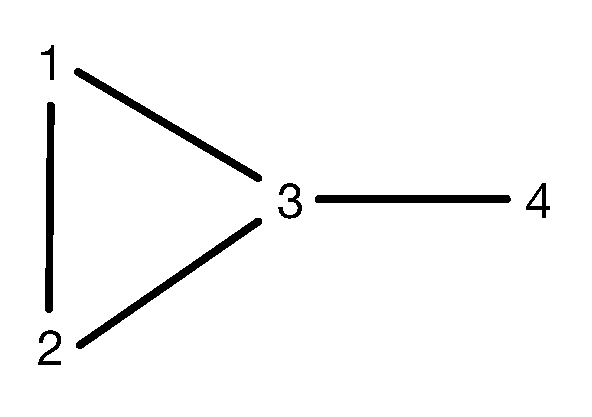
\includegraphics[scale=.5]{../figures/final-graph.pdf}
\end{center}
i.e. $G = (\{1,2,3,4\}, \{(1,2), (2,3), (3,1), (3,4)\})$.
\begin{enumerate}
\item List the bases and circuits of the graphic matroid $M_G = (E, I)$ for $G$.
\item Write down a list of inequalities describing the matroid polytope of $M_G$. \textbf{Hint: }\footnote{You should be able to get away with only 5 inequalities apart from the nonnegativity constraints, but it's ok if you write more.}
\item Let $I' = \{F \subset E:  d_F(3) \leq 2\}$. That is, $I'$ is the set of subgraphs of $G$ with at most $2$ edges incident to the vertex $3$. Write down a list of inequalities describing the polytope
$$ \conv(1_F: F \in I \cap I').$$
\end{enumerate}


\newpage 
Blank page

\newpage

\end{enumerate}




\end{document}
